\documentclass[border=0.8ex,svgnames,tikz]{standalone}
\usepackage{amsmath,mathtools}
\usepackage{fontspec}
\setmainfont{Source Serif 4}
\setsansfont{Source Sans 3}
\setmonofont{Source Code Pro}
\begin{document}
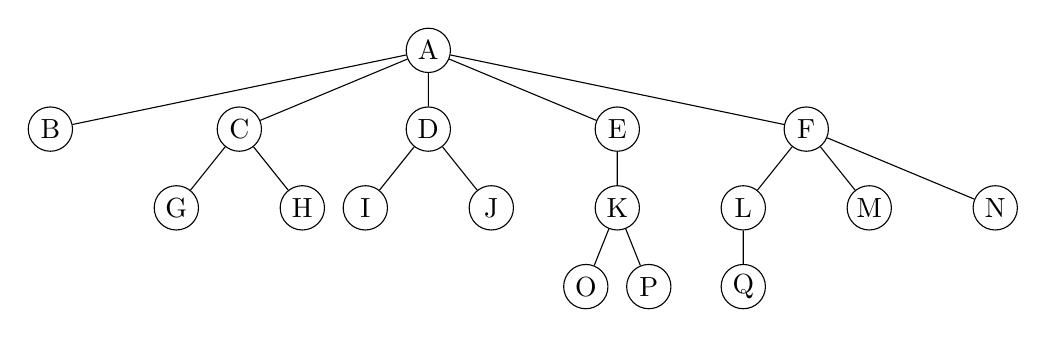
\begin{tikzpicture}[
  level distance=10mm,
  % every node/.style={fill=Red!64,circle,inner sep=1pt,minimum size=1.6em},
  % level 1/.style={sibling distance=24mm,nodes={fill=Red!45}},
  % level 2/.style={sibling distance=16mm,nodes={fill=Red!30}},
  % level 3/.style={sibling distance=8mm,nodes={fill=Red!12}},
  every node/.style={draw,circle,inner sep=1pt,minimum size=1.6em},
  level 1/.style={sibling distance=24mm},
  level 2/.style={sibling distance=16mm},
  level 3/.style={sibling distance=8mm},
  ]
  \node{A}
  child{ node{B} }
  child{ node{C} child{ node{G} } child{ node{H} } }
  child{ node{D} child{ node{I} } child{ node{J} } }
  child{
    node{E}
    child{ node{K} child{ node{O} } child{ node{P} } }
  }
  child{
    node{F} child[missing]
    child{ node{L} child{ node{Q} } }
    child { node{M} }
    child { node{N} }
  };
\end{tikzpicture}
\end{document}
